%% LyX 2.1.4 created this file.  For more info, see http://www.lyx.org/.
%% Do not edit unless you really know what you are doing.
\documentclass{beamer}
\usepackage{hyperref}
\usepackage{animate}
\usepackage{graphicx}
\def\Put(#1,#2)#3{\leavevmode\makebox(0,0){\put(#1,#2){#3}}}
\usepackage{color}
\usepackage{tikz}
\usepackage{amssymb}

\newcommand\blfootnote[1]{%
  \begingroup
  \renewcommand\thefootnote{}\footnote{#1}%
  \addtocounter{footnote}{-1}%
  \endgroup
}

\definecolor{LightGray}{gray}{0.9}

\ifx\hypersetup\undefined
  \AtBeginDocument{%
    \hypersetup{unicode=true,
 bookmarksnumbered=false,bookmarksopen=false,
 breaklinks=false,pdfborder={0 0 0},colorlinks=false}
  }
\else
  \hypersetup{unicode=true,
 bookmarksnumbered=false,bookmarksopen=false,
 breaklinks=false,pdfborder={0 0 0},colorlinks=false}
\fi

\makeatletter
%%%%%%%%%%%%%%%%%%%%%%%%%%%%%% Textclass specific LaTeX commands.
 % this default might be overridden by plain title style
 \newcommand\makebeamertitle{\frame{\maketitle}}%
 % (ERT) argument for the TOC
 \AtBeginDocument{%
   \let\origtableofcontents=\tableofcontents
   \def\tableofcontents{\@ifnextchar[{\origtableofcontents}{\gobbletableofcontents}}
   \def\gobbletableofcontents#1{\origtableofcontents}
 }

%%%%%%%%%%%%%%%%%%%%%%%%%%%%%% User specified LaTeX commands.
\usetheme{Malmoe}
% or ...
\useoutertheme{infolines}
\addtobeamertemplate{headline}{}{\vskip2pt}

\setbeamercovered{transparent}
% or whatever (possibly just delete it)



\setbeamertemplate{footline}
{
  \leavevmode%
  \hbox{%
  \begin{beamercolorbox}[wd=.5\paperwidth,ht=2.25ex,dp=1ex,center]{title in head/foot}%
    \usebeamerfont{title in head/foot}\insertshorttitle
  \end{beamercolorbox}%
  \begin{beamercolorbox}[wd=.5\paperwidth,ht=2.25ex,dp=1ex,right]{date in head/foot}%
    \usebeamerfont{date in head/foot}\insertshortdate{}\hspace*{2em}
    \insertframenumber{} / \inserttotalframenumber\hspace*{2ex} 
  \end{beamercolorbox}}%
  \vskip0pt%
}

\makeatother

\begin{document}

\title[Parallel detection of movement patterns]{Parallel Detection of Movement Patterns in Large Spatio-temporal Datasets}
%\author{Andres Calderon}
%\institute{University of California, Riverside}

\makebeamertitle

% \AtBeginSection[]{
%   \frame<beamer>{ 
%     \frametitle{Agenda}   
%     \tableofcontents[currentsubsection] 
%   }
% }

\newif\iflattersubsect

\AtBeginSection[] {
    \begin{frame}<beamer>
    \frametitle{Outline} %
    \tableofcontents[currentsection]  
    \end{frame}
    \lattersubsectfalse
}

\AtBeginSubsection[] {
    % \iflattersubsect
    \begin{frame}<beamer>
    \frametitle{Outline} %
    \tableofcontents[currentsubsection]  
    \end{frame}
    % \fi
    % \lattersubsecttrue
}

\begin{frame}{Trajectory datasets}
  \begin{minipage}{.5\textwidth}
    \begin{itemize}
    \item Sensors, sensors everywhere!!! 
    \item Anything that could move, will be tracked...
    \item Some applications:
        \begin{itemize}
         \item Social behavior
         \item Ecology (birds, sharks, ...)
         \item Climate change (icebergs, cyclones, ...)
         \item Software...
        \end{itemize}
    \end{itemize}
  \end{minipage}\begin{minipage}{.5\textwidth}
    \centering 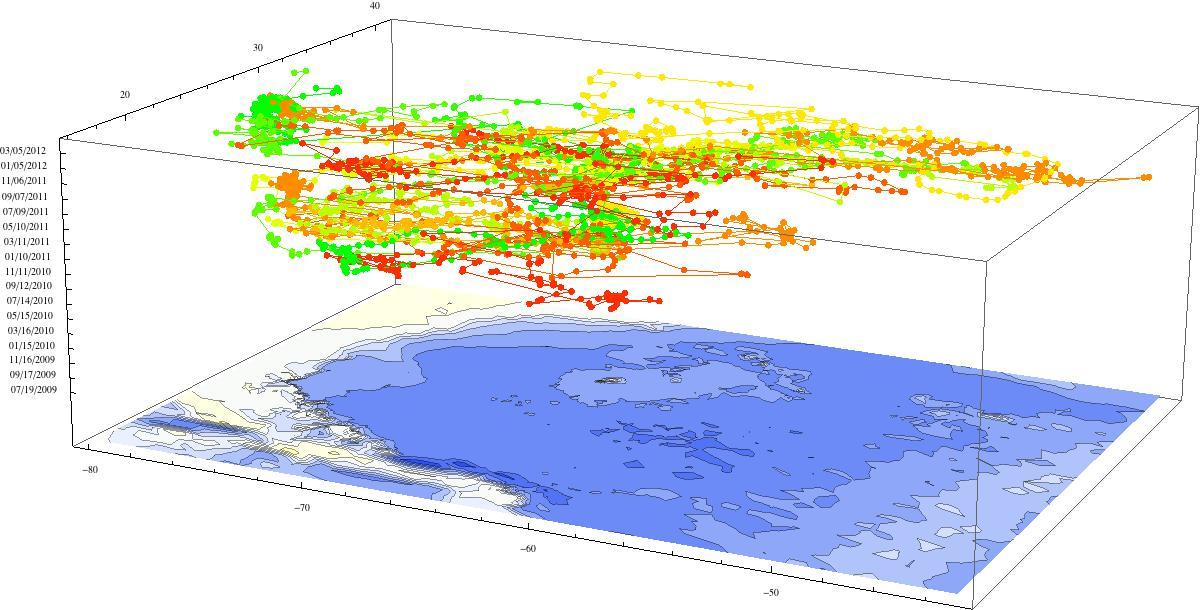
\includegraphics[width=0.75\textwidth]{Figures/sharks.jpg} \\
    \vspace{0.5cm}
    \centering 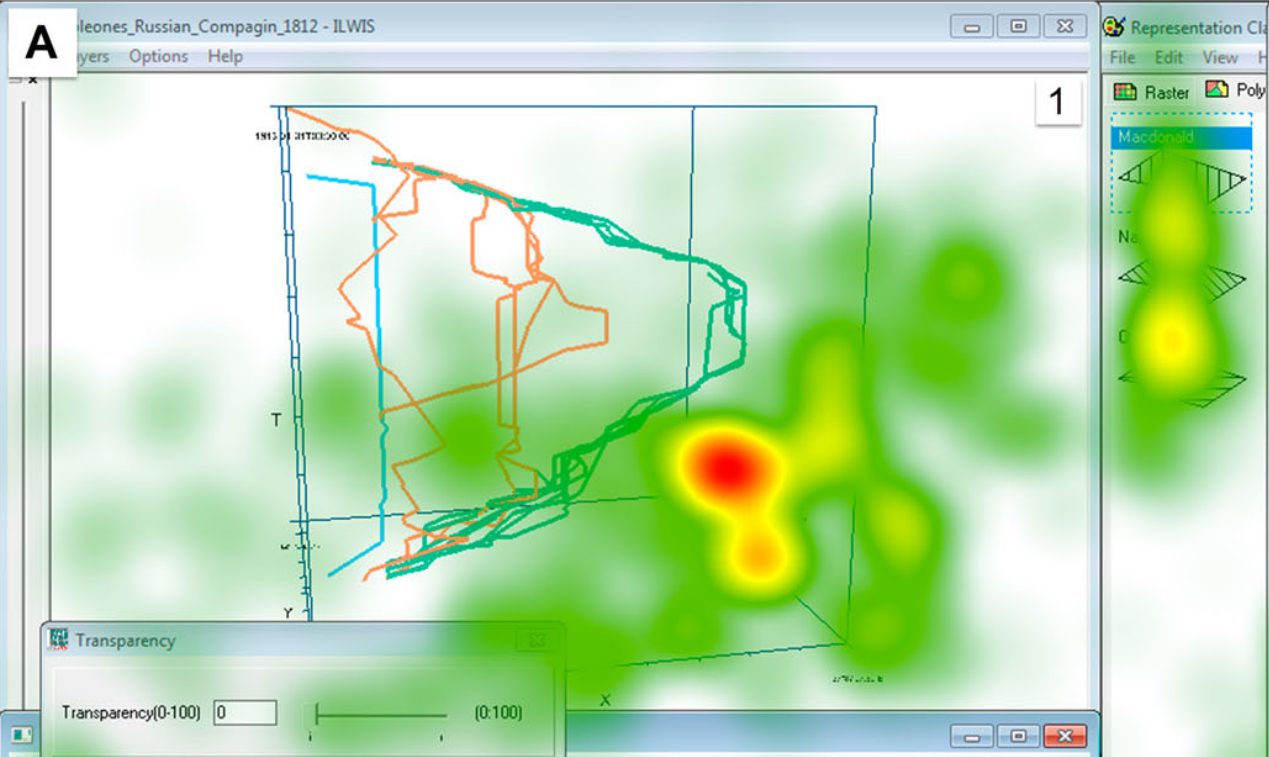
\includegraphics[width=0.75\textwidth]{Figures/eye.png}
  \end{minipage}
\end{frame}

\begin{frame}{Complex movement patterns}
  \begin{minipage}{.5\textwidth}
    Previous works focus on traditional queries:
        \begin{itemize}
            \item Range, Nearest Neighbors, Similarity, ...
        \end{itemize}
    Recent works look for the aggregate behavior:
        \begin{itemize}
            \item Moving clusters, Convoys, \textbf{Flocks}, Swarms, Gatherings, ...
        \end{itemize}
  \end{minipage}\begin{minipage}{.5\textwidth}
    \centering 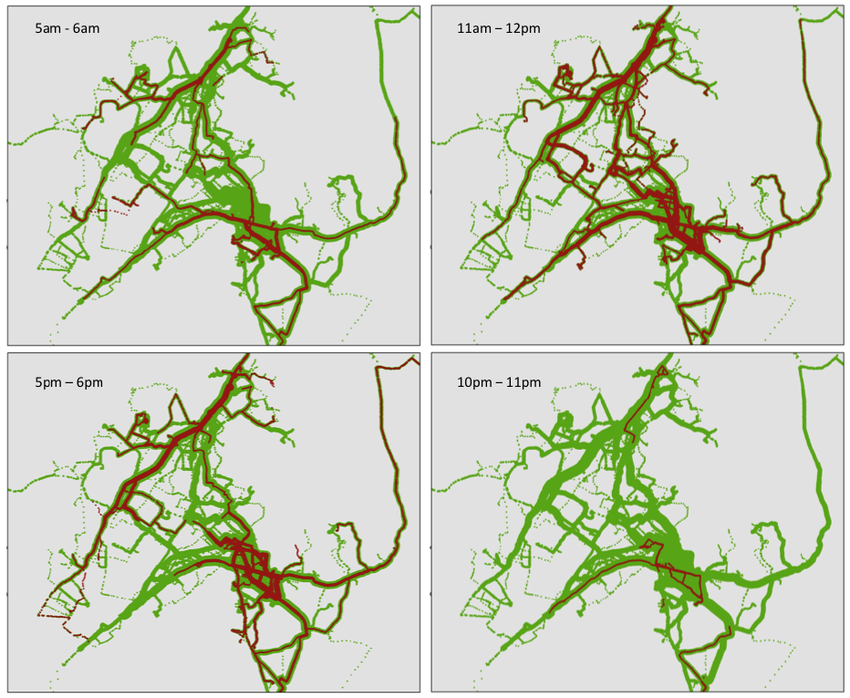
\includegraphics[width=0.6\textwidth]{Figures/similarity.png} \\
    \vspace{0.5cm}
    \centering 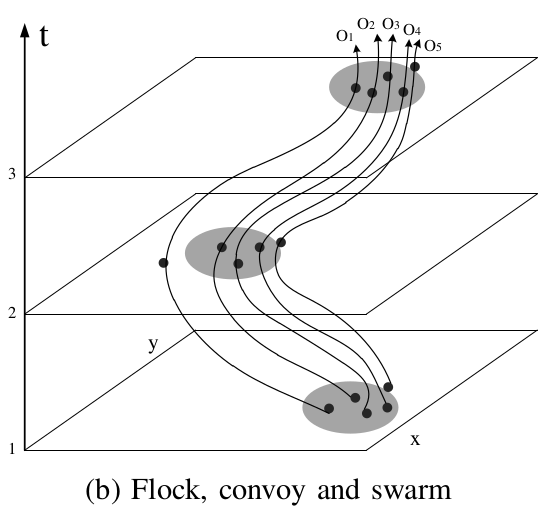
\includegraphics[width=0.6\textwidth]{Figures/cmp1.png}
  \end{minipage}
\end{frame}

\begin{frame}{What is a flock???} 
\small
  \begin{definition}[$(\mu,\varepsilon,\delta)-flock$]
    Sets of at least \alert{ $\mu$ } objects moving close enough (\alert{ $\varepsilon$ }) for at least \alert{ $\delta$ } time intervals (Benkert et al, 2008).
  \end{definition}
  \centering 
\includegraphics[page=2,height=0.4\textheight]{Figures/flock/f10}
  \begin{itemize}
   \item Vieira et al. (2009) proposed BFE algorithm (first polinomial solution).
   \item Drawbacks: 
    \begin{enumerate}
     \item Find disks is costly. They can be at any place.
     \item Huge amount of duplicate and redundant disks.
     \item Join between time intervals was a Cartesian product.
    \end{enumerate}
  \end{itemize}
\end{frame}

\begin{frame}{Contributions}
\small
  \begin{minipage}{.5\textwidth}
    \begin{enumerate}
     \item Boost the detection of disks through a parallel approach (spatial partitioning + expansions).
     \item Apply a frequent pattern mining approach to improve disk filtering (local + merge approach).
     \item Use parallel distance joins to improve combination between consecutive time intervals (a Distance parameter).
    \end{enumerate}


  \end{minipage}\begin{minipage}{.5\textwidth}
    \centering 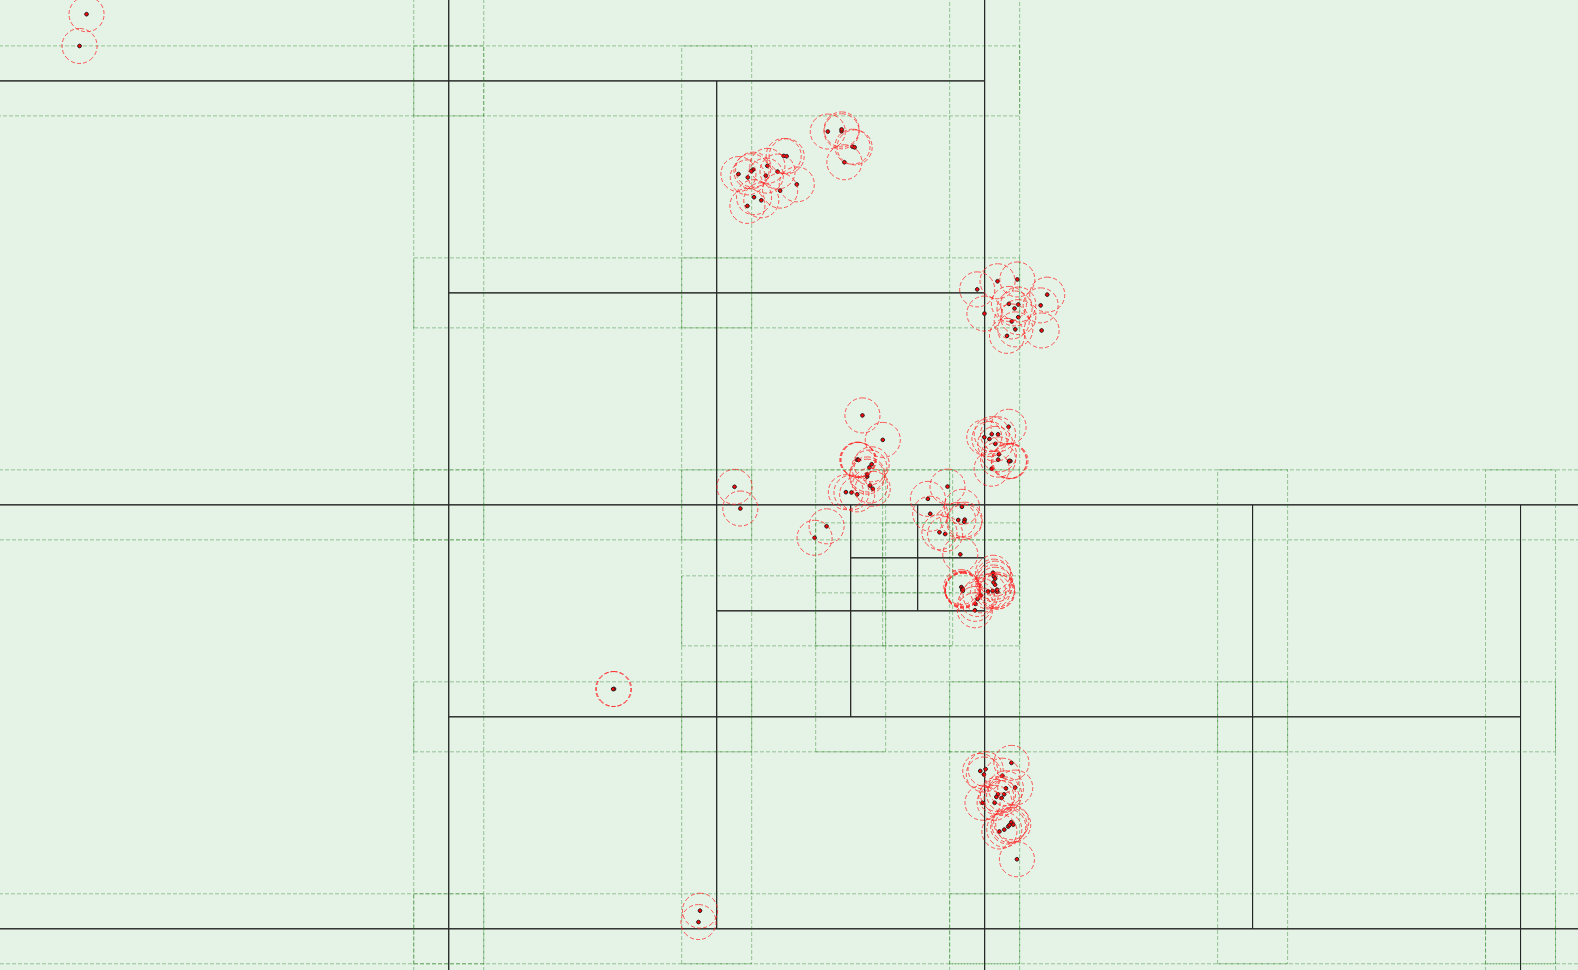
\includegraphics[width=0.8\textwidth]{Figures/centers.png} \\
    \vspace{0.5cm}
    \centering 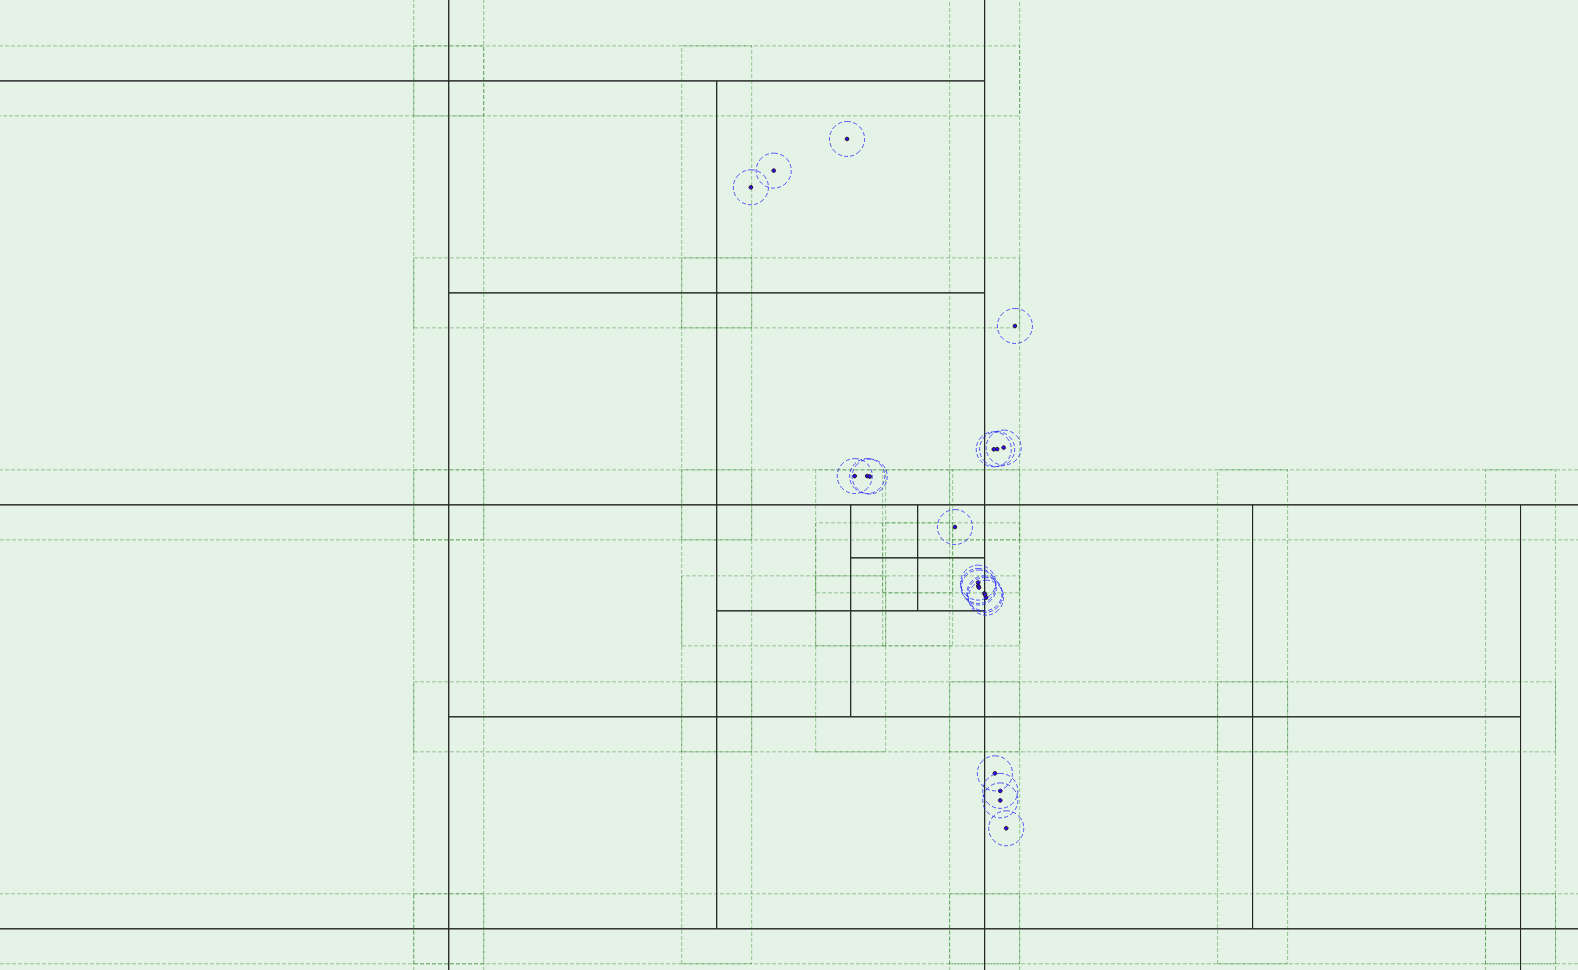
\includegraphics[width=0.8\textwidth]{Figures/disks.png}
  \end{minipage}
\end{frame}

\begin{frame}{Preliminar results} 
\small
    \begin{itemize}
        \item Implementation using GeoSpark. Synthetic datasets using SUMO (Simulation of Urban Mobility).
        \item Berlin network (OSM).  $\approx20K$ points per timestamp, 10 timestamps. Varying $\varepsilon$ ($\mu=3$ and $\delta=3$).
    \end{itemize}

  \centering 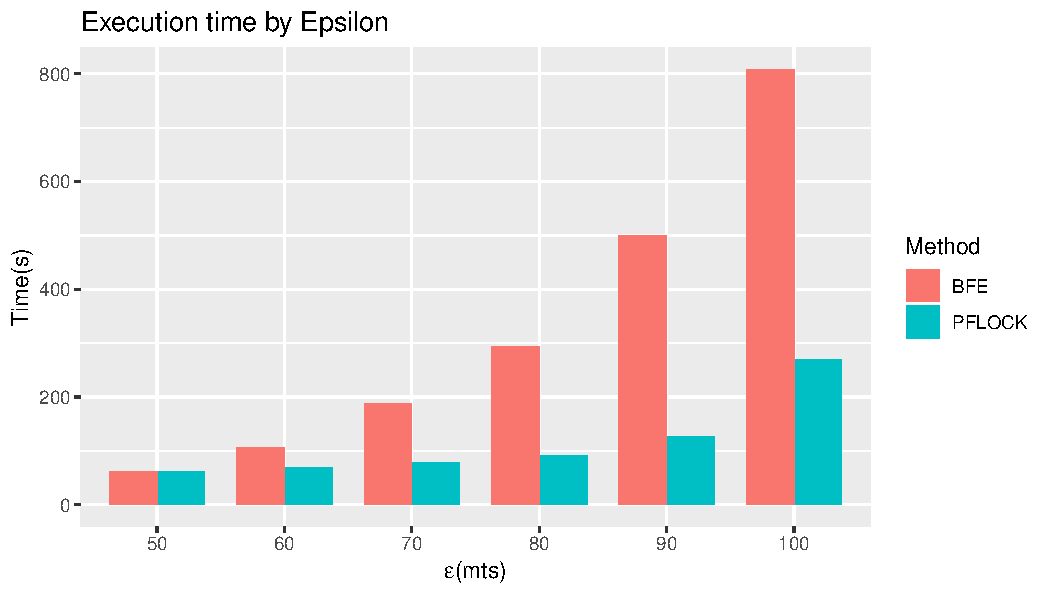
\includegraphics[width=0.9\textheight]{Figures/BFEvsPFLOCK2}
\end{frame}

\end{document}
